\subsection{Ultraschallsensor HC-SR04}
Diese Messung wird gemeinsam mit Gruppe 39 durchgeführt. \\
Ein sehr verbreitetes Modul für die Distanzmessung mittels Ultraschall ist 
das Modul HC-SR04. Dieses misst Distanzen mittels der Laufzeit von Schall. 
Dazu wird ein Ultraschall Impuls ausgesendet. Dieser wird von einem Objekt in 
der Umgebung reflektiert. Die Reflektion wird mit einem Ultraschallempfänger 
aufgefangen und in ein digitales Signal umgewandelt. 
\begin{figure}[h!]
    \centering
    \begin{tikztimingtable}
        Trigger     & L0.25C10C\\
        Ultraschall & 1.25L16{0.25c}5L;[gray]16{0.25c};L\\
        Echo        & 3.25L7CC\\
    \end{tikztimingtable}
    \label{tim_dist}
    \caption{Zeitdiagramm der Ansteuerung des Ultraschallsensors HC-SR04}
\end{figure}
Aufgrund der Länge dieses 
digitalen Signals und der Schallgeschwindigkeit kann nund die Distanz des 
Objekts bestimmt werden. 
\[ D = \frac{T \cdot c_{Luft}}{2} \]
\begin{tabular}{@{}ll}
    $D$         & Distanz \\
    $T$         & Pulsweite des Signals \\
    $c_{Luft}$  & Schallgeschwindigkeit in Luft \\
\end{tabular} \\
Mit diesem Sensor werden Messungen durchgeführt, um festzustellen, 
ob es geeignet ist, einen Eimer zu detektieren. 

\subsubsection{Messmittel}
\begin{table}[h!]
    \centering
    \begin{zebratabular}{lll}
        \rowcolor{gray} Gerät &
            Typ &
            Nummer \\
        Speisegerät &
            Hameg 8040 &
            SN 409128765 \\
        Oszilloskop &
            Agilent MSO6052A &
            Inv. Nr. 45; S/N: MY44001905 \\
        Pulsgenerator &
            Hameg 8035 &
            Inv. Nr. 44 \\
        Mainframe &
            Hameg 8001 &
            Inv. Nr. 108 \\
    \end{zebratabular} \\
    \caption[Messmittel Messungen HC-SR04]{Messmittel}
\end{table}
Die Messungen werden im Raum B332c durchgeführt. 

\subsubsection{Ansteuerung}
\begin{table}[h!]
    \centering
    \begin{zebratabular}{ll}
        \rowcolor{gray} Pin & Beschreibung \\
        VCC     & +5V DC \\
        Trig    & Trigger-Eingang (Startsignal) \\
        Echo    & Echo-Feedback \\
        GND     & Masse (0V) \\
    \end{zebratabular}
    \caption[Pinbelegung HC-SR04]{Pinbelegung}
\end{table}

\subsubsection{Testeimer}
Als Testeimer wird der Abfalleimer aus dem Raum C200 verwendet. \\
\begin{table}[h!]
    \centering
    \begin{zebratabular}{ll}
        \rowcolor{gray} Eigenschaft & Wert \\
        Durchmesser oben    & 38 cm \\
        Durchmesser unten   & 33 cm \\
        Höhe                & 48 cm \\
        Farbe               & Schwarz (matt) \\
        Material            & Kunststoff () \\
        Hersteller          & Helit \\
        Typ                 & 61062 \\
    \end{zebratabular}
    \caption{Definition Testeimer}
\end{table}

\subsubsection{Messung Messgenauigkeit}
Die folgenden Werte sind statistisch aus mindestens 1000 Einzelmessungen 
ermittelt. \\
\begin{table}[h!]
    \centering
    \begin{zebratabular}{lll}
        \rowcolor{gray} Abstand [cm] & Impuls mean [ms] & Std. Dev. [$\mu$s] \\
        50  & 2.987 & 2.4 \\
        60  & 3.503 & 2.4 \\
        70  & 4.060 & 10 \\
        80  & 4.766 & 24 \\
        90  & 5.230 & 10 \\
        100 & 5.807 & 11 \\
        110 & 6.413 & 13 \\
        120 & 7.040 & 16 \\
        130 & 7.722 & 22 \\
        140 & 8.229 & 16 \\
        150 & 8.854 & 15 \\
        160 & 9.500 & 43 \\
        170 & 10.06 & 22 \\
        180 & n.a.  & n.a. \\
    \end{zebratabular} \\
    \caption[Messwerte Messgenauigkeit HC-SR04]{Messwerte Messgenauigkeit}
\end{table}
Anschliessend wird eine weitere Messung durchgeführt. Dabei wird eine 
Holzplatte mit einem Abstand von 180 cm verwendet. Als Platte dient ein Regalbrett 
aus dem Raum B332c. Der Median beträgt 10.45 ms bei einer Standardabweichung 
von 9.7 $\mu$s. \\
$\to$ Deutlich besseres Signal auf flachen Gegenständen als auf Runden. 

\subsubsection{Messung seitliche Empfindlichkeit}
Um die seitliche Empfindlichkeit zu testen, wird der Eimer unter einem 
bestimmten Winkel vor dem Sensor aufgestellt. Der Abstand wird dabei 
so eingestellt, dass der Sensor den Eimer gerade noch erkennt. Die erzielte
Distanz wird gemessen. \\
Zwischen 25$^\circ$ und 30$^\circ$ hat der Sensor in einem Abstand von 75 bis 
90 cm einen blinden Bereich, in welchem der Eimer nicht erkannt wird. \\
\begin{minipage}{\textwidth}
\begin{minipage}{0.5\textwidth}
    \centering
    \begin{zebratabular}{ll}
        \rowcolor{gray} Winkel [$^\circ$] & Messbereich [cm] \\
        0   & 180 \\
        5   & 123 \\
        10  & 120 \\
        15  & 119 \\
        20  & 113 \\
        25  & 106 \\
        30  & 104 \\
        35  & 77  \\
        40  & 0   \\
    \end{zebratabular} \\
    \captionof{table}
        [Messwerte seitliche Empfindlichkeit HC-SR04]
        {Messwerte \\ seitliche Empfindlichkeit}
\end{minipage}
\begin{minipage}{0.5\textwidth}
    \centering
    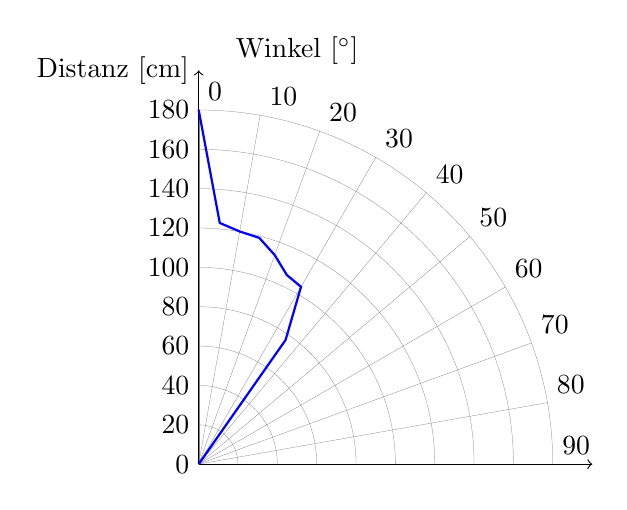
\begin{tikzpicture}[scale=2.5]
        % Grid
        % Grid for Angle
        \foreach \i in {0, 10, ..., 90}
        {
            \draw[ultra thin, gray] 
                (90-\i:0) -- (90-\i:1.8) 
                node[above right, black] {\i};
        }
        % Grid for Distance
        \foreach \i in {0, 20, ..., 180}
        {
            \draw[ultra thin, gray] 
                (0.01*\i,0) arc [radius = 0.01*\i, start angle = 0, end angle = 90] 
                node[left, black] {\i};
        }
        % Axis
        \draw[->] (0:0) -- (0:2);
        \draw[->] (0:0) -- (90:2) node[left] {Distanz [cm]};
        \node at (0.5, 2.1) {Winkel [$^\circ$]};
        % Data
        \draw[thick, blue]
            (90 - 0  : 1.80) -- 
            (90 - 5  : 1.23) -- 
            (90 - 10 : 1.20) -- 
            (90 - 15 : 1.19) -- 
            (90 - 20 : 1.13) -- 
            (90 - 25 : 1.06) -- 
            (90 - 30 : 1.04) -- 
            (90 - 35 : 0.77) -- 
            (90 - 40 : 0.00) ; 
    \end{tikzpicture}
    \captionof{figure}
        [Diagramm seitliche Empfindlichkeit HC-SR04]
        {Diagramm \\ seitliche Empfindlichkeit}
\end{minipage}
\end{minipage}

\subsubsection{Fazit}
Der Sensor ist nicht geeignet, um den Eimer zu finden, da der Sensor über 
einen zu breiten und zu ungenau definierten Winkel empfindlich ist. Der 
HC-SR04 wird somit nicht weiter als Sensor zur Detektion des Eimers 
weiterverfolgt. 

